\newcommand{\etas}{\ensuremath{\eta_{\mathrm{s}}}}


\chapter{Introduction}



Solar energy has been the key to the evolution of life on our planet earth, the existence of mankind and its advancement throughout the years. The human race has been utilizing solar energy in one way or another, actively or passively for survival and development purposes. Solar energy is abundant, free of cost and available to men throughout their lifetime. From point of view of environmental impact, it is the cleanest form of energy which is available on earth. While its counterpart fossil fuels like coal, natural gas, diesel, petrol and other petroleum products etc. is a major source of global pollution and Environmental degradation.
% These days fossil fuels are exploited to meet energy demand by all the countries and it is being depleted at a very fast pace. Since it is limited, the situation is alarming and it will get worse as time progresses. As all the countries are progressing, every single day demand of these fossil fuels is increasing. Increasing demand leads to depletion of fossil fuel which is rising at an exponential rate. It is direct and a very serious threat to the environment of the planet earth in the form of pollution and global warming.	

% It is of paramount importance to protect and maintain the habitable stature of the earth for the sake of mankind.
Limited availability of fossil fuel and its role in environmental deterioration makes this necessary that its consumption should be replaced at least partially if not completely by cleaner source of energy like solar energy. As it resolves both the issues of availability and environmental protection, It is the best way to move forward with. According to Kalogirou\citep{KALOGIROU2004231}, Global yearly energy demand is equal to the solar energy falling on earth for just 30 minutes, only if it is utilized completely. one of the ways of harnessing solar energy is through using different solar thermal applications. Different types of solar thermal appliances have been developed to trap solar energy which can be used in the industry and drop down the use of the conventional source of energy. Few examples are flat plate collector, parabolic trough collector, cylindrical collector, paraboloidal dish collector, linear Fresnel collector etc. All of these collect solar radiation over a large area and use it for the heating purpose which can be further utilized.

% Apart from environmental issues, study and research in the field of solar thermal application are required for national security as well. One of the most important aspects of the national security of a sovereign country is energy security. Energy security of any country can not stand solely on fossil fuel. Its limited availability demands research and development for different sources of energy. Thus, to ensure energy security of a country consistent work in the area of solar thermal applications is required. Many researchers have worked in this field for developments of tools needed for trapping and utilizing solar energy.

Various studies have been performed to understand underlying physics and to make these energy conversions more efficient. Since performing these studies with experiments is costly and time-consuming, researchers use computer models to simulate the physical model as an alternative to experiments. With the advancement in computer science and its calculative power, it is cheaper and quicker to perform a simulation of a physical model and analyze the results rather than performing experiments. Various subtle changes in the simulation can be studied easily without much effort. These pros of numerical simulation make it more viable option for further study and research on the topic. 

Many of the solar thermal systems like linear Fresnel collector, dish collector etc. contain cavity receivers. Thus an understanding of different processes associated within cavity become important. These cavity receivers are used to heat up the working fluid for industrial processes. Thus the understanding of modes of heat losses from cavities is very important. There are three modes of heat transfer which are- conduction, convection and radiation. Radiation and convection play important role in heat losses from a cavity to surroundings while all the three modes are involved in the flow of heat within the cavity. Different modes of heat transfer within and from cavity receiver have been illustrated in the figure\ref{modeht}. 

\begin{figure}[H]
\begin{center}
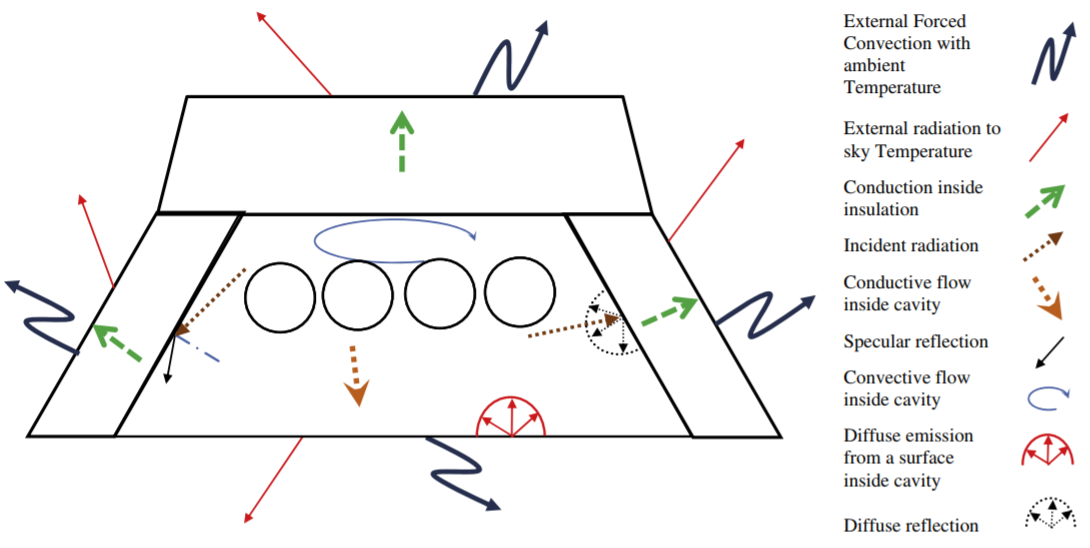
\includegraphics[width=0.8\textwidth]{modeHT.PNG}
\caption{Modes of heat transfer from a cavity receiver\citep{MOGHIMI2015343}}
\end{center}
\label{modeht}
\end{figure}

It is advantageous to study how heat is lost to the surroundings via radiation and convection and what are the elements facilitating these losses. After good understanding of losses and the factors controlling it, the design of cavity can be modified and improvement in efficiency and performance can be made. These studies also help in the study of temperature distribution within the cavity. Whether it contains hot spots or not, which is an important factor from the design point of view. Numerical studies can help improve the design to get rid of such flaws and make the overall design better. It helps in quantifying these losses and further minimizing them. Detailed study of convection and radiation has been done in the literature.  A lot of work has been done in this field where researchers have studied and quantified heat losses associated with cavities. Experimental and numerical studies have been performed for convective and radiative heat losses for cavities used in parabolic dish collectors by Prakash et al.\citep{PRAKASH2009157} and Shavazi et al.\citep{ABBASISHAVAZI2015269}. Similar studies have been performed for a cavity with two stage concentrators and compared with numerical studies performed using CFD package FLUENT 6.2 by Reddy and Kumar\citep{Reddy2009}. Recently Robert et al.\citep{doi:10.1063/1.4949066} have worked towards reducing the convective losses from cavity using experiments and CFD tools.

This report contains studies performed on the cavity receivers, mainly square cavity and trapezoidal cavity used with linear Fresnel reflector and various simulation conducted on it. It includes findings of these simulations and experiments. Further, it contains validation of numerical schemes to be used for future work with benchmarked solutions and finally, future work to be done.
